\documentclass[12pt]{article}
\usepackage{parskip}
\usepackage[a4paper, total={6.25in, 9in}]{geometry}
\usepackage{amsmath,amsfonts,amsthm,bm}
\usepackage[english]{isodate}
\usepackage[final]{pdfpages}
\usepackage{graphicx} 
\usepackage{breakcites}
\usepackage{mathtools}
\usepackage[displaymath, mathlines]{lineno}
\usepackage[labelfont=bf,skip=0.5cm,justification=justified,singlelinecheck=false]{caption}
\bibliographystyle{apalike}
%%%%%%%%%%%%%%%%%%%%%%%%%%%%%%%%%%%%%%%%%%%%%%%%%%%%%%%%%%%%%%%%%%%%%%%%%%%%%%%%%%%%
%% Stuff for line numbering %%%%%%%%%%%%%%%%%%%%%%%%%%%%%%%%%%%%%%%%%%%%%%%%%%%%%%%%
%%%%%%%%%%%%%%%%%%%%%%%%%%%%%%%%%%%%%%%%%%%%%%%%%%%%%%%%%%%%%%%%%%%%%%%%%%%%%%%%%%%%
\newcommand*\patchAmsMathEnvironmentForLineno[1]{%
  \expandafter\let\csname old#1\expandafter\endcsname\csname #1\endcsname
  \expandafter\let\csname oldend#1\expandafter\endcsname\csname end#1\endcsname
  \renewenvironment{#1}%
     {\linenomath\csname old#1\endcsname}%
     {\csname oldend#1\endcsname\endlinenomath}}% 
\newcommand*\patchBothAmsMathEnvironmentsForLineno[1]{%
  \patchAmsMathEnvironmentForLineno{#1}%
  \patchAmsMathEnvironmentForLineno{#1*}}%
\AtBeginDocument{%
\patchBothAmsMathEnvironmentsForLineno{equation}%
\patchBothAmsMathEnvironmentsForLineno{align}%
\patchBothAmsMathEnvironmentsForLineno{flalign}%
\patchBothAmsMathEnvironmentsForLineno{alignat}%
\patchBothAmsMathEnvironmentsForLineno{gather}%
\patchBothAmsMathEnvironmentsForLineno{multline}%
}
%%%%%%%%%%%%%%%%%%%%%%%%%%%%%%%%%%%%%%%%%%%%%%%%%%%%%%%%%%%%%%%%%%%%%%%%%%%%%%%%%%%
%%%%%%%%%%%%%%%%%%%%%%%%%%%%%%%%%%%%%%%%%%%%%%%%%%%%%%%%%%%%%%%%%%%%%%%%%%%%%%%%%%%

\title{Controls on genotype entropy in dispersive environments}
\author{\small{Burcu Tepekule, Gregory Britten}}
\date{\small{\printdayoff\today}}

\begin{document}
\maketitle 
%\linenumbers

\subsection*{Abstract}
Motivated by models of marine microbial diversity, we investigate the forces acting on the distribution of genotypes in a dispersive environment. Integrating patch dynamics and mutator-replicator theory, we demonstrate the opposing forces of dispersal, selection, and mutation controlling the distribution of genotypes across connected environments of variable fitness. 

Hypotheses: local Shannon entropy is controlled by the following forces:
\begin{itemize}
\item \textbf{Selection acting to reduce local entropy via competitive exclusion}. At zero dispersal with no mutation, species in isolated environments approach competitive exclusion with the most fit genotypes approaching fixation.  
\item \textbf{Mutation generates entropy within-environments}. Mutation leads to survival of the flattest.
\item \textbf{Dispersal mixes entropy across environments}. Infinite dispersal with  or without mutation collapses the meta-environmental structure and leads to competitive exclusion with respect to the mean environment, or also complete neutrality in the 'no free lunch' scenario. At intermediate dispersal, a mutation-selection-dispersal balance emerges wherein suboptimal genotype distributions arise due to mixing of environments. High dispersal leads to survival of the flattest. 
\end{itemize}

Throughout the paper we characterize genotype distributions in terms of the Shannon entropy within and across environments.
\subsection*{Questions}

\begin{itemize}
\item \textbf{mutation-selection balance} How does the entropy distribution change as a function of 1) mutation rate, 2) dispersal rate, 3) selection gradient ($\alpha\delta r$), 4) dispersal network structure (degree distribution), 

\item \textbf{Species interactions} Is `few strong many weak` robust to dispersal network structure? Are other interaction networks more robust for particular dispersal networks? Mutualism vs. antagonism; conjugate interaction-dispersal matrix pairs
\item \textbf{Complexity versus stability}
\end{itemize}

\subsection*{Binary sequences}
\begin{align*}
X_{000} &= [0,0,0]\\
X_{001} &= [0,0,1]\\
\vdots \\
X_{111} &= [1,1,1]\\
\end{align*}

With three bits we have $2^n$ sequences.


\subsection*{Governing ordinary differential equation}

The governing ODE for the logistic quasispecies on a dispersal network is as follows 

\[ \frac{dx_{i}^{l}}{dt} = r_i^l x_i^l\left(1 - \frac{\Sigma x^l}{k_i^l}\right) 
		 + \sum_{\substack{j\\j \neq i}}^N q^{h(i,j)}x_j^l
		 - \sum_{\substack{j\\j \neq i}}^N q^{h(i,j)}x_i^l
		 + \sum_{\substack{k\\k \neq l}}^{P}m_{i}^{k \rightarrow l}x_{i}^{k}		
		 -  \sum_{\substack{k\\l \neq k}}^{P}m_{i}^{l \rightarrow k} x_{i}^{l} \] 

with parameters and state variable symbols defined in Table X. 

\begin{table}[!h]
\centering
   \caption{Parameter and state variance definitions for the governing ODE} 
\begin{tabular}{lll}
 \textbf{Symbol} &  \textbf{Definition}  \\
 $r_i^l$           & intrinsic growth rate  \\
 $x_i^l$          & concentration of sequence $i$ in environment $l$  \\
 $\Sigma x^l $ & total sequence abundance in environment $l$  \\
 $k_i^l$      & carrying capacity of species $i$ in environment $l$ \\ 
 $q$            & mutation probability  per bit\\
 $h(i,j)$           & Hamming distance between sequences $i$ and $j$\\
 $N$               & Number of unique sequences per patch \\
 $m_i^{h\rightarrow l}$ & dispersal rate of species $i$ from patch $k$ to $l$\\
 $P$  & number of patches 
\end{tabular}
\end{table}

We write the system of ODEs in matrix-vector notation
\[ \frac{d \mathbf{x}}{dt} = \mathbf{R\Sigma x}  
		 + \mathbf{Qx}
		 + \mathbf{Mx}\] 
		 
where
\[ \mathbf{R} = \begin{bmatrix}
    r_1^1 & 0        & \dots & \dots & \dots & 0  \\
           0 & r_2^1 & \ddots & \ddots & \ddots & 0 \\
   \vdots & \ddots & \ddots & \ddots & \ddots & \vdots \\
   \vdots & \ddots & \ddots &  r_1^2 & \ddots & \vdots  \\
   \vdots & \ddots & \ddots & \ddots & \ddots   & \vdots \\
           0 &         0 &  \dots  & \dots  & \dots & r_N^P \\ \end{bmatrix} \]
           
\[ \mathbf{\Sigma} = \begin{bmatrix}
    (1-\frac{\Sigma x^1}{k_1^1}) & 0        & \dots & \dots & \dots & 0  \\
           0 & (1-\frac{\Sigma x^1}{k_2^1}) & \ddots & \ddots & \ddots & 0 \\
   \vdots & \ddots & \ddots & \ddots & \ddots & \vdots \\
   \vdots & \ddots & \ddots &  (1-\frac{\Sigma x^2}{k_1^2}) & \ddots & \vdots  \\
   \vdots & \ddots & \ddots & \ddots & \ddots   & \vdots \\
           0 &         0 &  \dots  & \dots  & \dots & (1-\frac{\Sigma x^P}{k_N^P}) \\ \end{bmatrix} \]

\[ \mathbf{Q} = \begin{bmatrix}
    0 & q^{h(1,2)}  & \dots & q^{h(1,N)} & 0 & \dots & \dots & 0 & \dots & 0 \\
 q^{h(2,1)} & 0   & \dots & q^{h(2,N)} & 0 & \dots & \dots & 0 & \dots & 0\\
   \vdots & \vdots & \ddots & \vdots & \vdots   & \vdots & \vdots & \vdots & \dots & \vdots\\
       q^{h(N,1)} &  q^{h(N,2)} &   \dots  & 0  & 0 & \dots & \dots & 0 & \dots & 0 \\ 
       0 & 0 & \dots &  0 & 0 & q^{h(1,2)}  & \dots & q^{h(1,N)} & \dots & 0\\
       0 & 0 & \dots &  0 & q^{h(2,1)} & 0 & \dots & q^{h(2,N)}&\dots&0\\
        \vdots & \vdots & \vdots &  \vdots & \vdots & \vdots & \ddots & \vdots & \dots & \vdots\\
          0 & 0 & \dots &  0 & q^{h(N,1)} & q^{h(N,2)} & \dots & 0 & \dots & 0\\	 
          \vdots & \vdots & \vdots & \vdots & \vdots & \vdots & \vdots & \vdots & \ddots & \vdots \\
          0 & 0 & \dots & 0 & 0 & 0 & \dots & 0 & \dots & 0\end{bmatrix}  \]

with $h(i,j) = h(j,i)$, and 

\[ \mathbf{M} = \begin{bmatrix}
    -m_1^{1\rightarrow 2} & 0        & \dots & m_1^{2\rightarrow 1} & 0 & \dots & m_1^{3\rightarrow 1} & 0 & \dots & 0  \\
           0 & -m_2^{1\rightarrow 2} & 0 & \dots & m_2^{2\rightarrow 1} & 0 &  \dots & m_2^{3\rightarrow 1} & \dots & 0 \\
   \vdots & 0& \ddots & \ddots & \dots & \vdots \\
   m_1^{1\rightarrow 2} & \vdots & \ddots &  -m^{} & \ddots & \vdots  \\
   0 & \ddots & \ddots & \ddots & \ddots   & \vdots \\
           0 &         0 &  \dots  & \dots  & \dots & (1-\Sigma x^P) \\ \end{bmatrix} \]

\subsection*{Steady state analysis}
For the purpose of notation, we define
\[ \frac{dx_{i}^{l}}{dt} \equiv f(x_{i}^{l}). \]

\subsection*{The Jacobian matrix}
\[ J_{i,j}^l = \frac{\partial f(x_i^l)}{\partial x_j^l}\Bigr|_{\substack{{x_i^l=x_i^l}^*\\{x_j^l=x_j^l}^*}}  \]

The general Jacobian matrix is then
\[ \mathbf{J} = \begin{bmatrix}
    \frac{\partial f(x_1^1)}{\partial x_1^1} & \frac{\partial f(x_1^1)}{\partial x_2^1} & \dots & \frac{\partial f(x_1^1)}{\partial x_N^1}  &  \frac{\partial f(x_1^1)}{\partial x_1^2} & \frac{\partial f(x_1^1)}{\partial x_2^2} & \dots & \frac{\partial f(x_1^1)}{\partial x_N^{P}} \\ 
    \frac{\partial f(x_2^1)}{\partial x_1^1} &  \frac{\partial f(x_2^1)}{\partial x_2^1} & \dots & \dots & \dots & \dots & \dots & \frac{\partial f(x_2^1)}{\partial X_N^P} \\
    \vdots    & \vdots & \ddots  & \ddots & \ddots & \ddots & \ddots & \vdots\\
    \frac{\partial f(x_N^1)}{\partial x_1^1} & \vdots   & \ddots  & \ddots & \ddots & \ddots & \ddots & \vdots \\
    \frac{\partial f(x_1^2)}{\partial x_1^1} & \vdots & \ddots  & \ddots & \ddots & \ddots & \ddots & \vdots \\
    \frac{\partial f(x_2^2)}{\partial x_1^1} & \vdots & \ddots  & \ddots & \ddots & \ddots & \ddots & \vdots\\
    \vdots   & \vdots & \ddots  & \ddots & \ddots & \ddots & \ddots & \frac{\partial f(x_{N-1}^P)}{\partial x_N^P}\\
    \frac{\partial f(x_N^P)}{\partial x_1^1} & \frac{\partial f(x_N^P)}{\partial x_1^2} & \dots & \dots & \dots & \dots & \frac{\partial f(x_N^P)}{\partial x_{N-1}^P} & \frac{\partial f(x_N^P)}{\partial x_N^P} \\    
\end{bmatrix} \]

where species $1:N$ in patch $l$ are stacked as the top rows, followed by species $1:N$ in patch $l+1$, and so on. 

\subsection*{Equations for the case $N = 2, P=2$}

\begin{align*}
\frac{dx_1^1}{dt} &=  r_1^1 x_1^1\left(1 - \frac{\Sigma x^1}{k_1^1}\right)  + qx_2^1 - qx_1^1+  m_1^{2\rightarrow 1} x_1^2 - m_1^{1\rightarrow 2} x_1^1\\
\frac{dx_2^1}{dt} &= r_2^1 x_2^1\left(1 - \frac{\Sigma x^1}{k_2^1}\right) + qx_1^1 - qx_2^1 + m_2^{2\rightarrow 1} x_2^2 - m_2^{1\rightarrow 2}x_2^1\\
\frac{dx_1^2}{dt} &=  r_1^2 x_1^2\left(1 - \frac{\Sigma x^2}{k_2^2}\right) + qx_2^2 - qx_2^1 + m_1^{1\rightarrow 2}x_1^1 - m_1^{2\rightarrow 1}x_1^2 \\
\frac{dx_2^2}{dt} &=  r_2^2 x_2^2\left(1 - \frac{\Sigma x^2}{k_2^2}\right) + qx_1^2 - qx_2^2 + m_2^{1\rightarrow 2} x_2^1 - m_2^{2\rightarrow 1} x_2^2\\
\end{align*}

So the Jacobian is 

\begin{align*}
\mathbf{J} &= \begin{bmatrix}
    \frac{\partial f(x_1^1)}{\partial x_1^1} & \frac{\partial f(x_1^1)}{\partial x_2^1} & \frac{\partial f(x_1^1)}{\partial x_1^2} & \frac{\partial f(x_1^1)}{\partial x_2^2}\\ 
        \frac{\partial f(x_2^1)}{\partial x_1^1} & \frac{\partial f(x_2^1)}{\partial x_2^1} & \frac{\partial f(x_2^1)}{\partial x_1^2} & \frac{\partial f(x_2^1)}{\partial x_2^2}\\ 
            \frac{\partial f(x_1^2)}{\partial x_1^1} & \frac{\partial f(x_1^2)}{\partial x_2^1} & \frac{\partial f(x_1^2)}{\partial x_1^2} & \frac{\partial f(x_1^2)}{\partial x_2^2}\\ 
                \frac{\partial f(x_2^2)}{\partial x_1^1} & \frac{\partial f(x_2^2)}{\partial x_2^1} & \frac{\partial f(x_2^2)}{\partial x_1^2} & \frac{\partial f(x_2^2)}{\partial x_2^2} \\    
\end{bmatrix} \\
 &= \scriptsize{\begin{bmatrix}
    r_1^1 - \frac{r_1^1}{k_1^1} \Sigma x^1 - q -  m_1^{1\rightarrow 2} &  
    	q & 
    		m_1^{2\rightarrow 1} & 
    			0 \\ 
    q & 
    	r_2^1 - \frac{r_2^1}{k_2^1}\Sigma x^1 - q - m_2^{1\rightarrow 2} & 
    		0 & 
    			m_2^{2\rightarrow 1} \\
    m_1^{1\rightarrow 2} & 
    	0 & 
    		r_1^2 - \frac{r_1^2}{k_1^2} \Sigma x^2 - q - m_1^{2\rightarrow 1}& 
    			q \\
    0 & 
    	m_2^{1\rightarrow 2} & 
    		q &
    			r_2^2 - \frac{r_2^2}{k_2^2} \Sigma x^2 - q - m_2^{2\rightarrow 1} \\       
\end{bmatrix} }
\end{align*}

We partition the Jacobian into intra-community interaction and meta-community dispersal components
\[ \mathbf{J} = \mathbf{J_{R\Sigma}} + \mathbf{J_Q} + \mathbf{J_M} \]

where
\begin{align*}
\mathbf{J_{R\Sigma}} &= \small{\begin{bmatrix}
    r_1^1 - \frac{r_1}{k_1^1}^1\Sigma x^1 & 0 & 0 & 0 \\ 
        0 & r_2^1 - \frac{r_2^1}{k_2^1} \Sigma x^1 & 0 & 0 \\
    0 & 0 & r_1^2 - \frac{r_1^2}{k_1^2}\Sigma x^2 & 0 \\
    0 & 0 & 0 & r_2^2 - \frac{r_2^2}{k_2^2} \Sigma x^2  \\       
\end{bmatrix}} \\
 \mathbf{J_Q} &= \begin{bmatrix}
    0 & q^{h(1,2)} & 0 & 0 \\ 
    q^{h(2,1)} & 0 & 0 & 0 \\
    0 & 0 & 0 & q^{h(1,2)} \\
    0 & 0 & q^{h(2,1)} & 0 \\       
\end{bmatrix} \\
 \mathbf{J_M} &= \begin{bmatrix}
    -m_1^{1\rightarrow 2} & 0 & m_1^{2\rightarrow 1} & 0 \\ 
    0 & -m_2^{1\rightarrow 2}& 0 & m_2^{2\rightarrow 1} \\
    m_1^{1\rightarrow 2} & 0 & -m_1^{2\rightarrow 1} & 0 \\
    0 & m_2^{1\rightarrow 2} & 0 & -m_2^{2\rightarrow 1} \\       
\end{bmatrix} 
\end{align*}

\subsection*{Shannon diversity}
Shannon diversity is simply the Shannon information entropy applied to the distribution of genotypes in the environment
\[ H = -\sum_{l \in P} \sum_{i \in l} p^l_i \log p^l_i  -  sum \]

where the $p_i^l \log p_i^l$ sum of is taken per genotype within environment $l$ and then taken with respect to the environmental mean and the 

We consider the disaggegared Shannon diversity for within-environment and across-environment, respectively
\[ H_w = -\sum_{i\in N} \langle p_i^l\rangle_l \log \langle p_i^l \rangle_l \]
\[ H_b = -\sum_{l\in P} \langle p_i^l\rangle_i \log \langle p_i^l \rangle_i \]

\subsection*{Classical ANOVA decomposition}
The within-between decomposition of entropy is made analogously to the classical ANOVA decomposition from statistics
\begin{align*} 
SS_{total} &= \sum_{l\in P} \sum_{i\in l}\left( x_i^l - \langle \langle x \rangle_i \rangle_l \right)^2 \\
                &= \sum_{i\in l} \left( x_i^l - \langle x^l \rangle_i \right)^2 + \sum_{i\in N} \left( \langle x^l \rangle_i - \langle \langle x \rangle_i \rangle_l \right)^2 \\
                &= SS_{within} + SS_{between}
\end{align*}

Similar to entropy, the hypothesis is that mutation, dispersal, and selection all contribute uniquely to these terms. Via generation of within-environment variance, mutation positively drives $SS_{within}$ upward, while selection directly opposes mutation via mutation-selection balance. Dispersal, on the other hand, positively drives $SS_{within}$ by effectively converting $SS_{between}$ to $SS_{within}$. Note that $SS_{between}$ can only be generated by in this model by variation in selection among environments. 

\subsection*{Genetic drift and neutral mutations}
Genetic drift is not included in this model, not the capacity for gene mutation to be selectively neutral and therefore contribute to genetic entropy. 

\subsection*{Competitive exclusion}
In a deterministic environment with no dispersal or mutation, the species with the highest carrying capacity (lowest R*)

\begin{align*}
\frac{dx_1}{dt} &= rx_1\left(1-\frac{\Sigma x}{k_1}\right)\\
\frac{dx_2}{dt} &= rx_2\left(1-\frac{\Sigma x}{k_2}\right)\\
\frac{dx_3}{dt} &= rx_3\left(1-\frac{\Sigma x}{k_3}\right)\\
\end{align*}

in which case the genotype with the largest $k$ will outcompete the others and go to fixation
\[ t \rightarrow \infty\implies \frac{x_{\max{k}}}{\Sigma x} \rightarrow 1 \]

and accordingly
\[\frac{x_{\max{k}}}{\Sigma x} \rightarrow 1 \implies H \rightarrow 0 \] 

Competitive exclusion dynamics for the 3 genotype system with no mutation and no dispersal is given in Figure X. 

\subsection*{Evolutionary tradeoffs}


\bibliography{library}
%%%%%%%%%%%%%%%%%%%%%%%%%%%%%%%%%%%%%%%%%%%%%%%%%%%%%%%%%%%%%%%%%%%%%%%%
%% Figures %%%%%%%%%%%%%%%%%%%%%%%%%%%%%%%%%%%%%%%%%%%%%%%%%%%%%%%%%%%%%
%%%%%%%%%%%%%%%%%%%%%%%%%%%%%%%%%%%%%%%%%%%%%%%%%%%%%%%%%%%%%%%%%%%%%%%%
\newpage
\begin{figure}

 \hspace*{-2cm}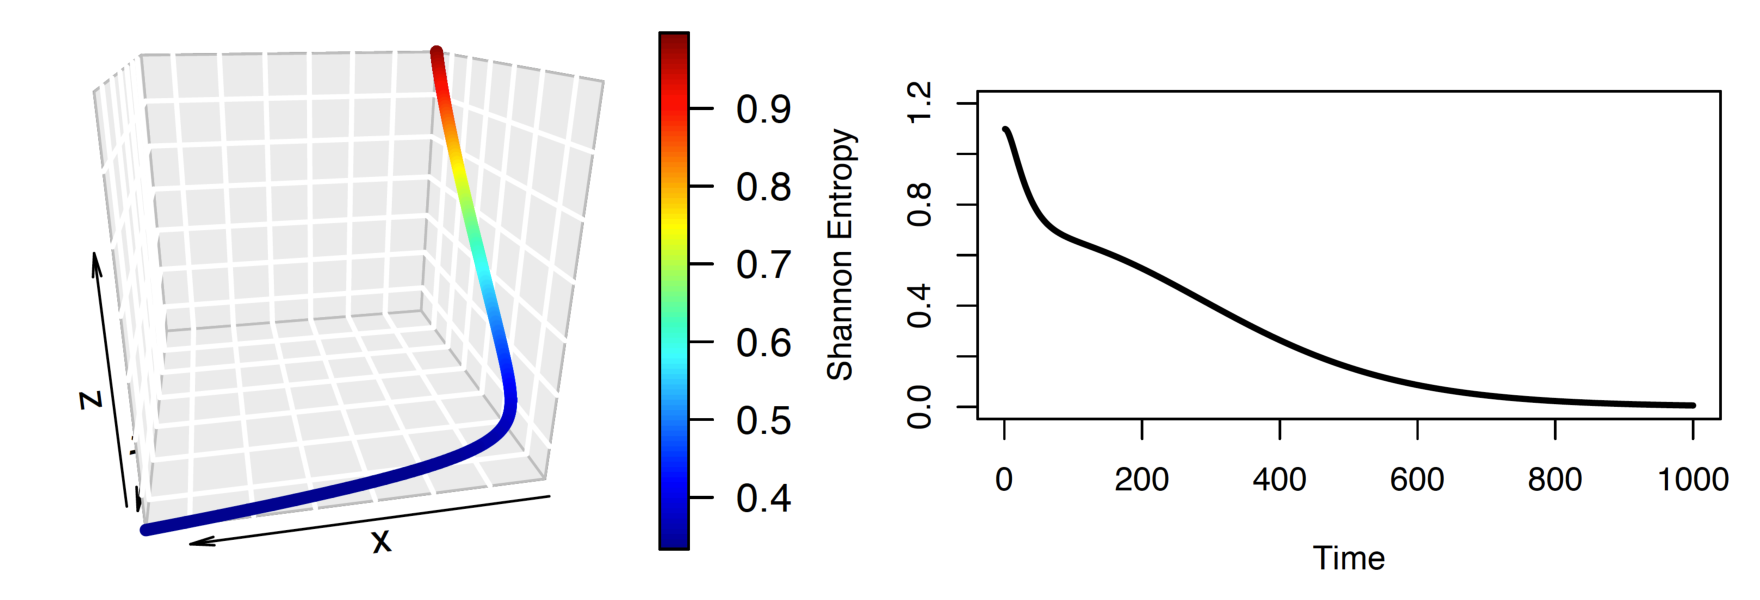
\includegraphics[scale=0.65]{entropy3d.pdf}
 \caption{Competitive exclusion among three genotypes in an environment with no dispersal and no mutation.}
\end{figure}

\newpage

\begin{figure}
 \hspace*{-1cm}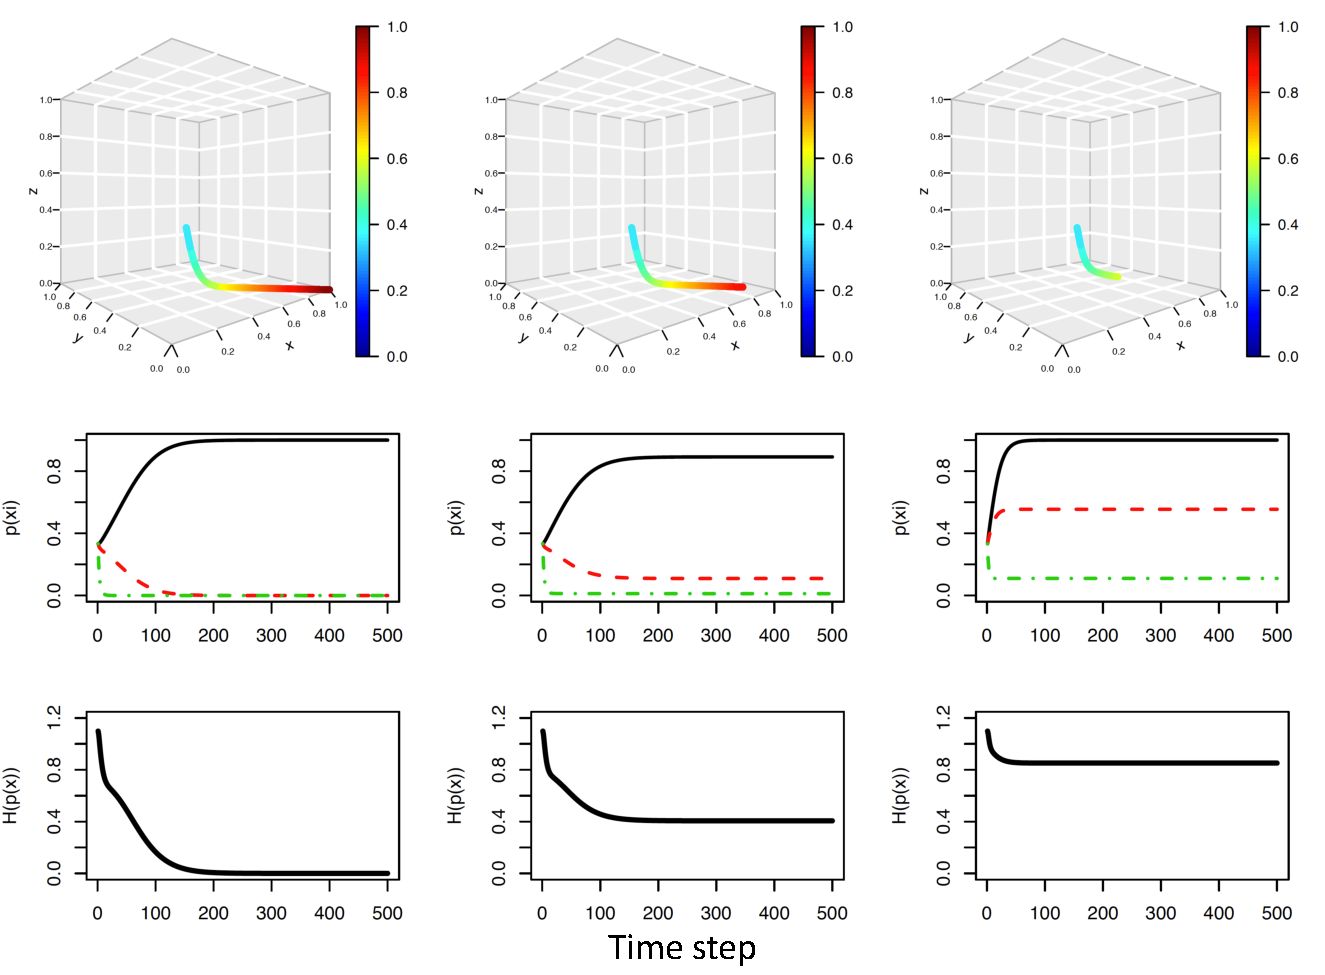
\includegraphics[scale=0.65]{entropy3x3.pdf}
 \caption{Competitive exclusion among three genotypes with and without mutation and no dispersal. Left column is with 0 mutation, while the middle and right columns give the steady state with $q=0.1$ and $q=1$, respectively.}
\end{figure}
 
 
\end{document}